% 5
\section{実験}

% 5.1
\subsection{環境}
プログラムの作成は、Unityを使って行った。これは Unity Technologies が開発を行っている、統合開発環境の名称である。ウェブプラグイン、デスクトッププラットフォーム、ゲーム機、携帯電話用OSなど、多岐にわたるプラットフォームに対応している。スクリプト言語として、C\#、 Javascript、 Boo を使用することができる。OpenCV はWebカメラから映像を取得する際に使用した。その他にも、画像の加工等の部分で使用した。

\begin{center}
  \begin{tabular}{|c|c|}\hline
    \raisebox{-0.2ex}{OS} & \raisebox{-0.2ex}{Windows 8.1 Enterprise 64bit} \\ \hline
    \raisebox{-0.2ex}{CPU} & \raisebox{-0.2ex}{Intel(R) Core(TM) i7-2600 CPU 3.40GHz} \\ \hline
    \raisebox{-0.2ex}{メモリ} & \raisebox{-0.2ex}{4.0GB} \\ \hline
    \raisebox{-0.2ex}{統合開発環境} & \raisebox{-0.2ex}{Unity 5.1.0} \\ \hline
    \raisebox{-0.2ex}{開発言語} & \raisebox{-0.2ex}{C\#} \\ \hline
    \raisebox{-0.2ex}{ライブラリ} & \raisebox{-0.2ex}{OpenCV 2.4.10} \\ \hline
    \raisebox{-0.2ex}{ウェブカメラ} & \raisebox{-0.2ex}{Logicool HD Webcam C270, Logicool HD Webcam C525} \\ \hline
  \end{tabular}
\end{center}

% 5.2
\subsection{実行結果}
Unity を用いて、3D空間にオブジェクトを配置する。実際にオブジェクトを配置した結果が図5-1、図5-2となる。

 \vspace{5mm}
\begin{minipage}{0.5\hsize}
  \begin{center}
   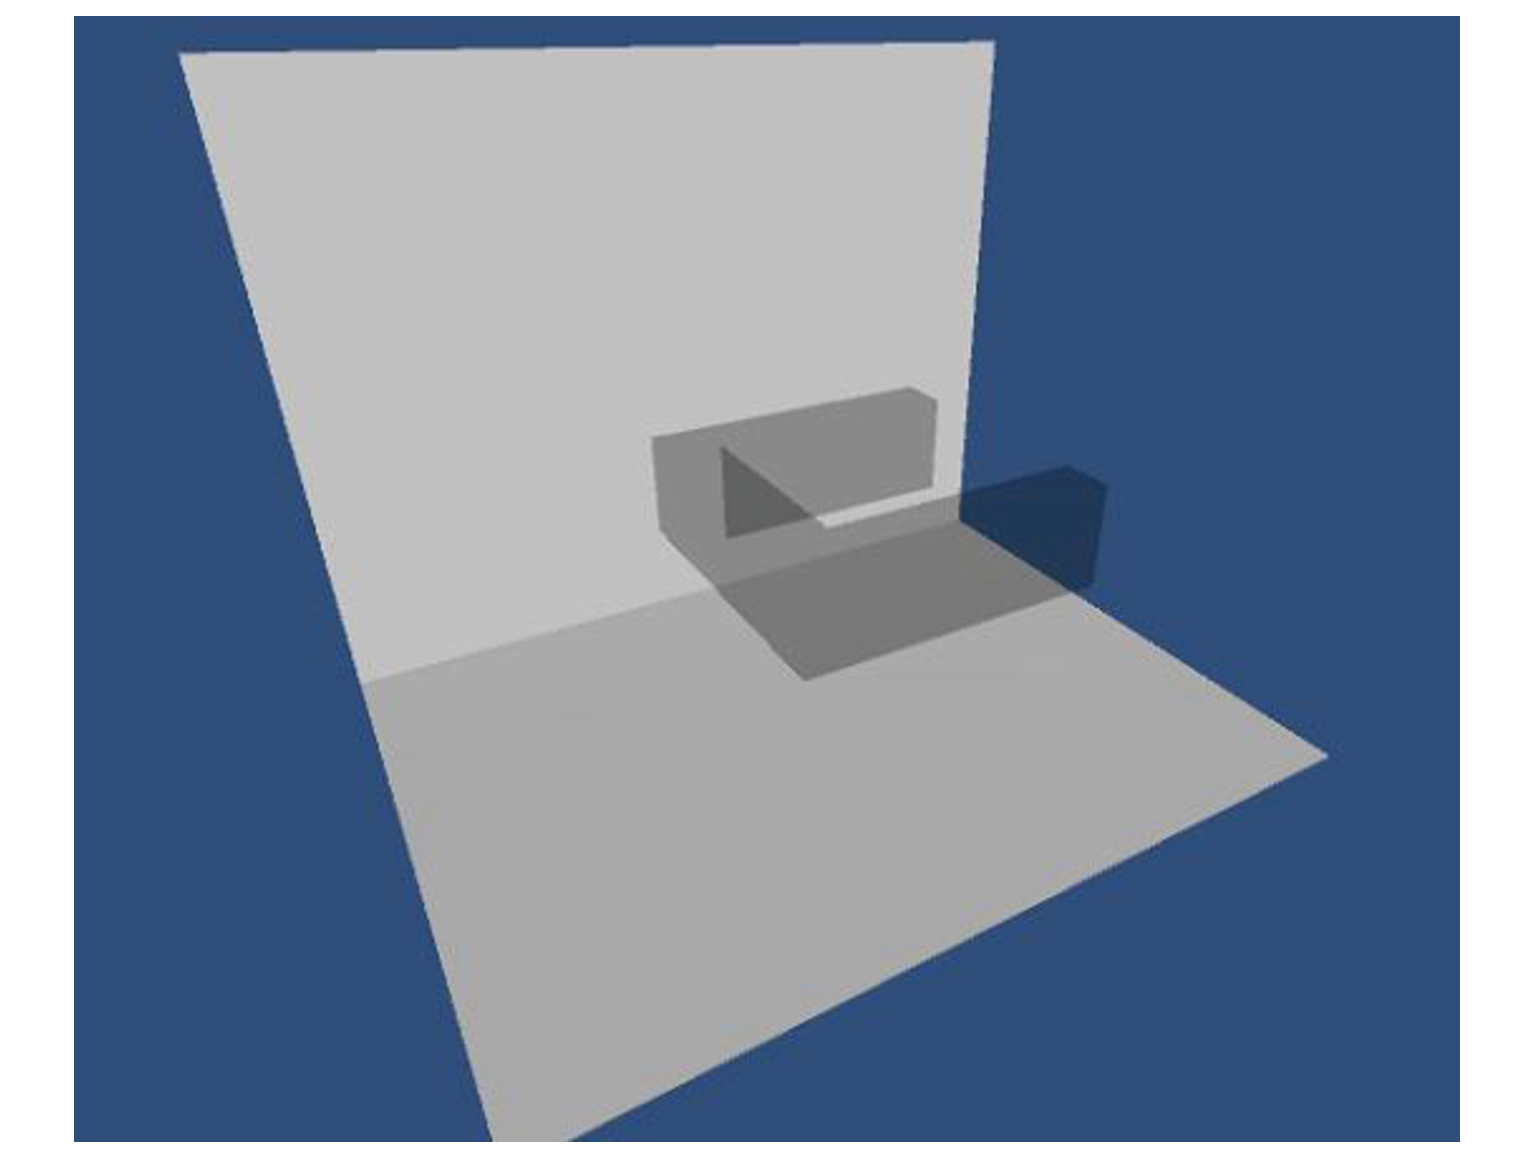
\includegraphics[width=70mm]{3d_obje_2.eps}
   図5-1. 作成した3Dオブジェクト
  \end{center}
  \label{fig:one}
 \end{minipage}
 \begin{minipage}{0.5\hsize}
  \begin{center}
   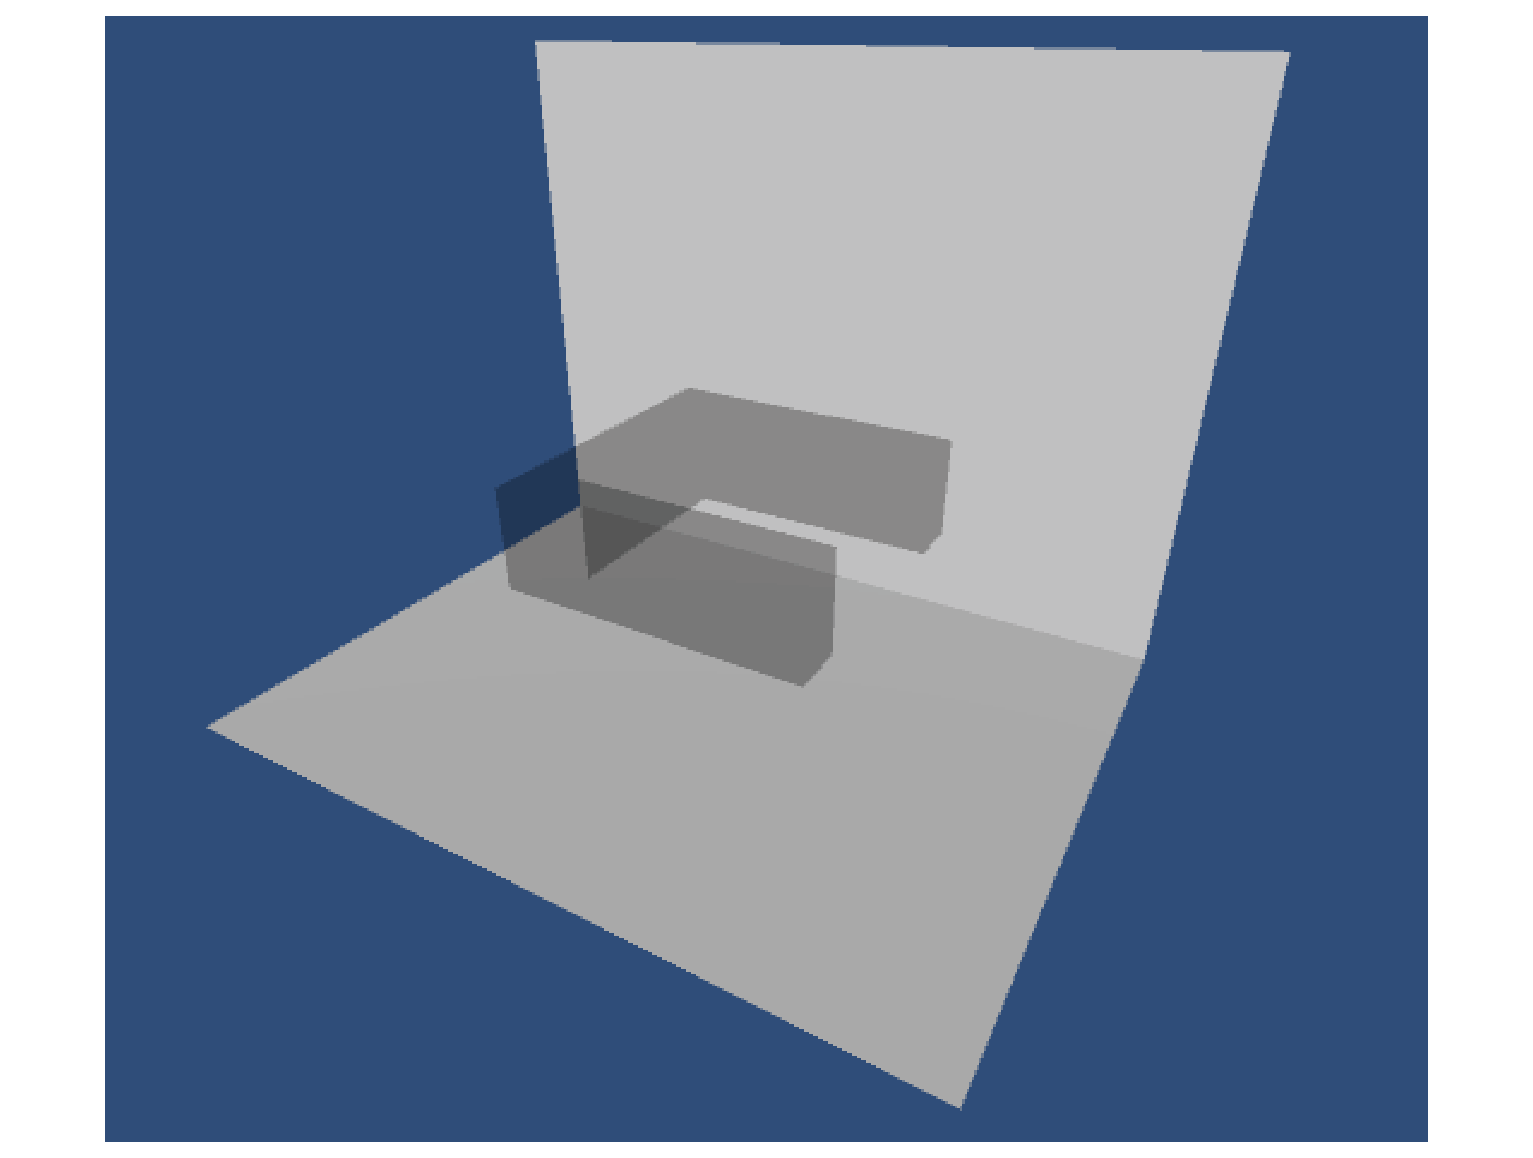
\includegraphics[width=70mm]{3d_obje_1.eps}
   図5-2. 作成した3Dオブジェクト
  \end{center}
  \label{fig:two}
 \end{minipage}

このオブジェクトに対して、3D格子点の内部外部判定を行う。結果は、図5-3となる。

 \vspace{5mm}
\begin{minipage}{0.5\hsize}
  \begin{center}
   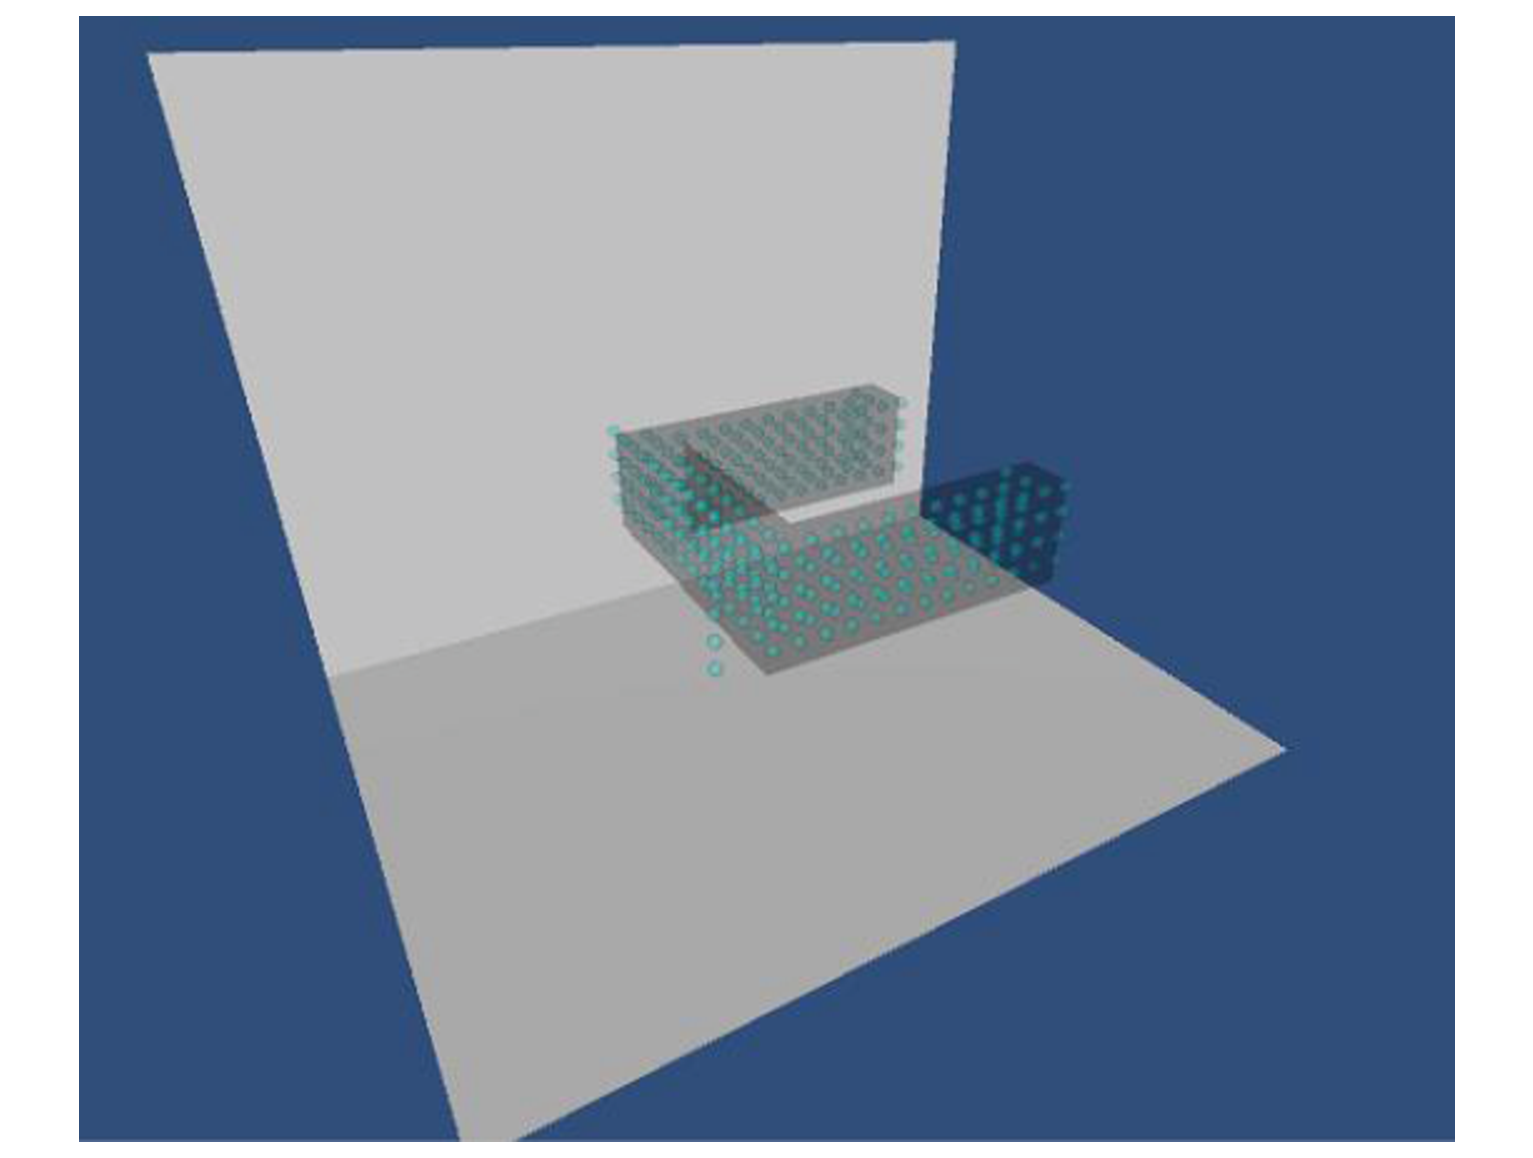
\includegraphics[width=70mm]{IED3D_2.eps}
   図5-3. 内部外部判定結果
  \end{center}
  \label{fig:one}
 \end{minipage}
 \begin{minipage}{0.5\hsize}
  \begin{center}
   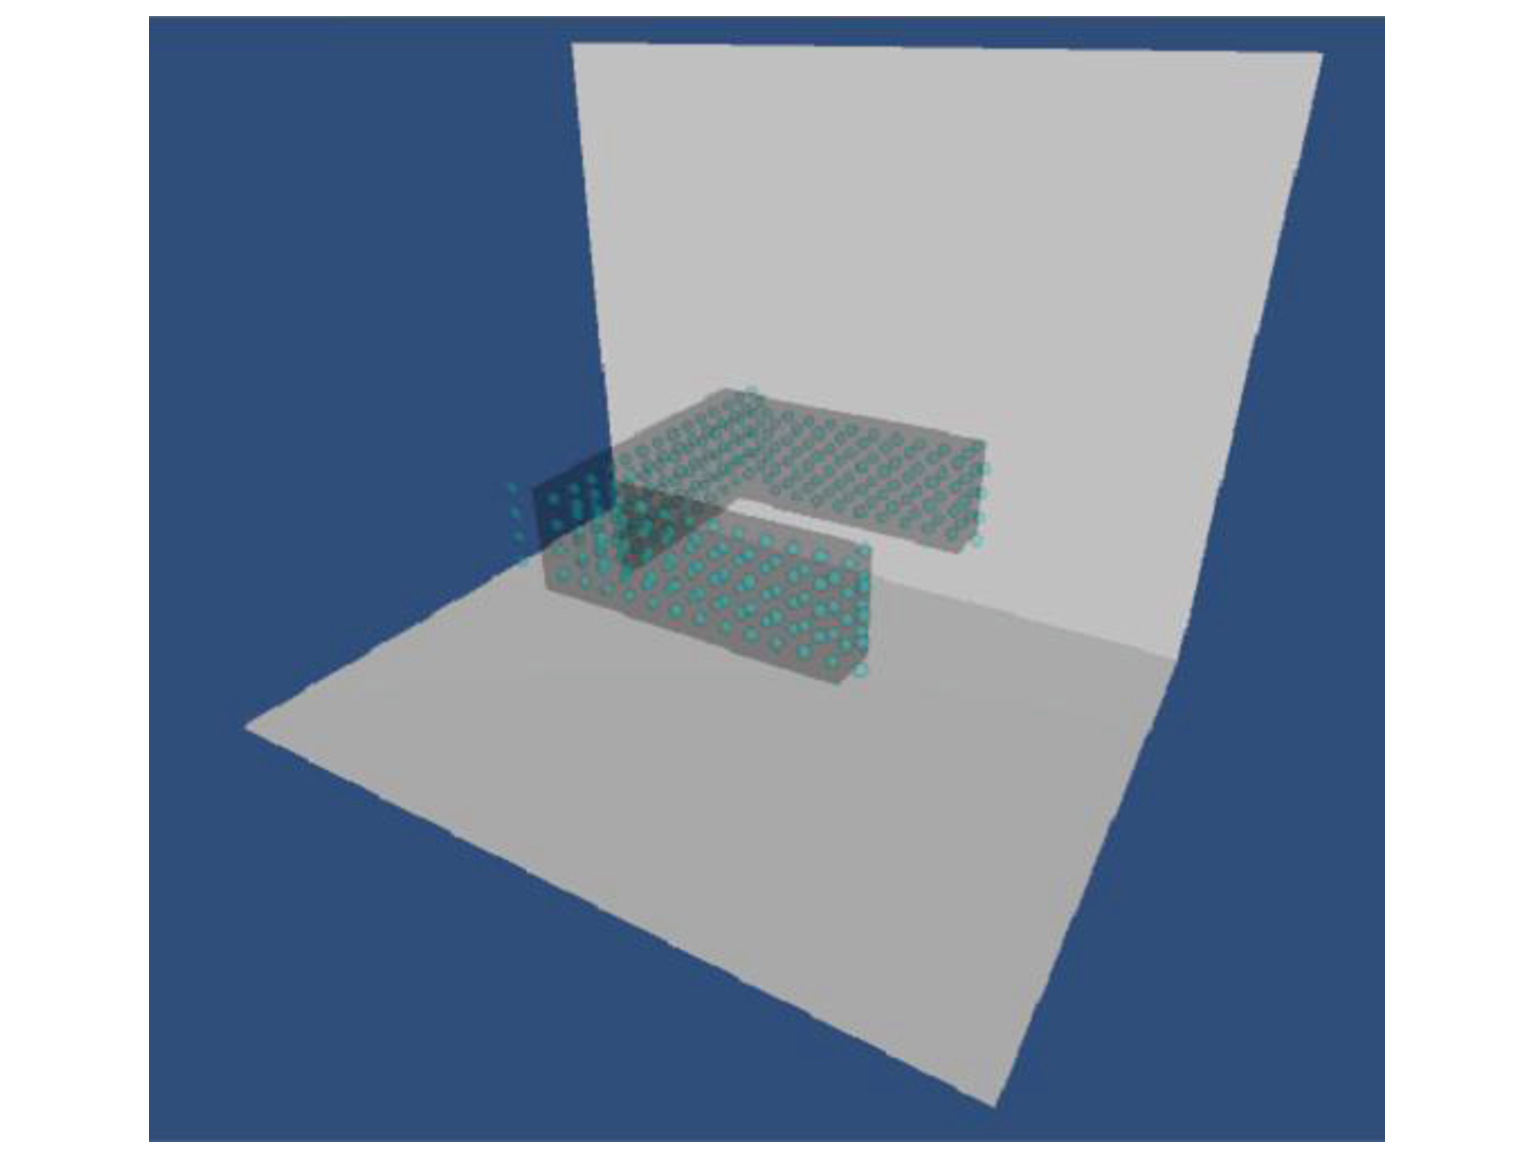
\includegraphics[width=70mm]{IED3D_1.eps}
   図5-4. 内部外部判定結果
  \end{center}
  \label{fig:two}
 \end{minipage}

青緑色の球が、内部と判定された格子点となる。若干の誤判定はあるが、概ね見た目通りに内部外部を判定できていることがわかる。ここで、3Dオブジェクトの窪んだ部分に手を挿入することで、内部外部判定を用いた当たり判定が正常に動作していることを確認する。

 \vspace{5mm}
\begin{minipage}{0.5\hsize}
  \begin{center}
   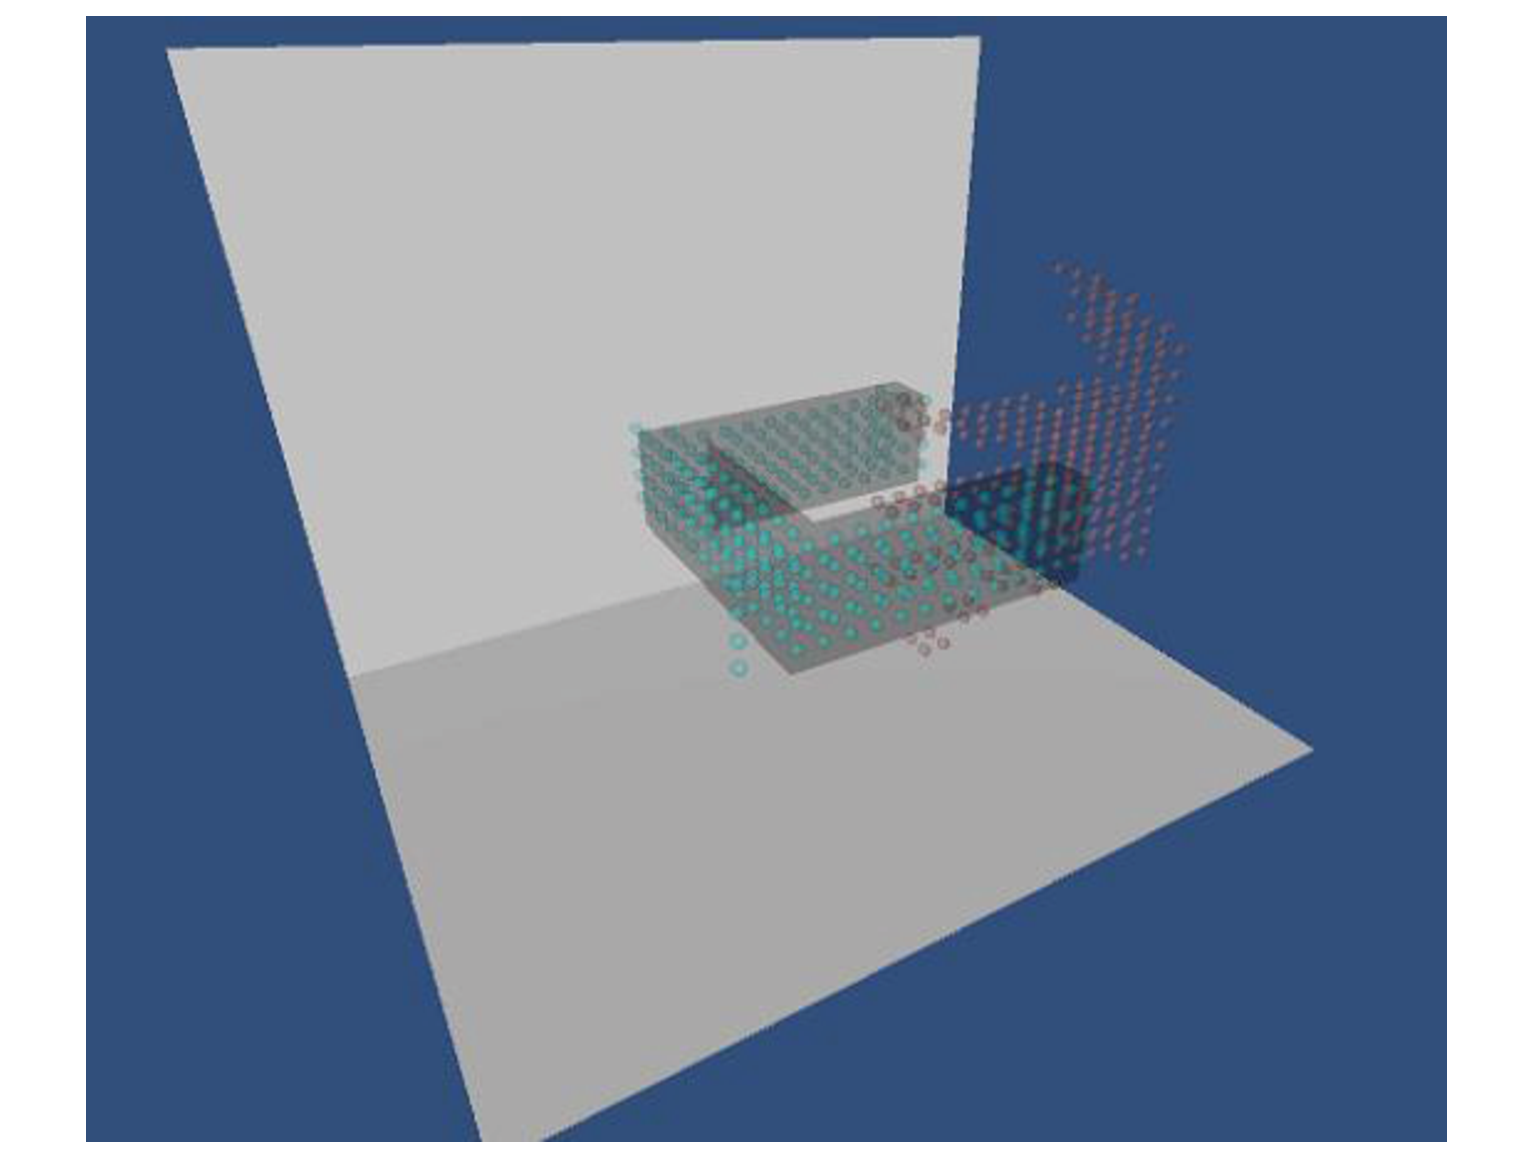
\includegraphics[width=70mm]{3D_obje_insert_1.eps}
   図5-5. 手をオブジェクトの窪みに挿入
  \end{center}
  \label{fig:one}
 \end{minipage}
 \begin{minipage}{0.5\hsize}
  \begin{center}
   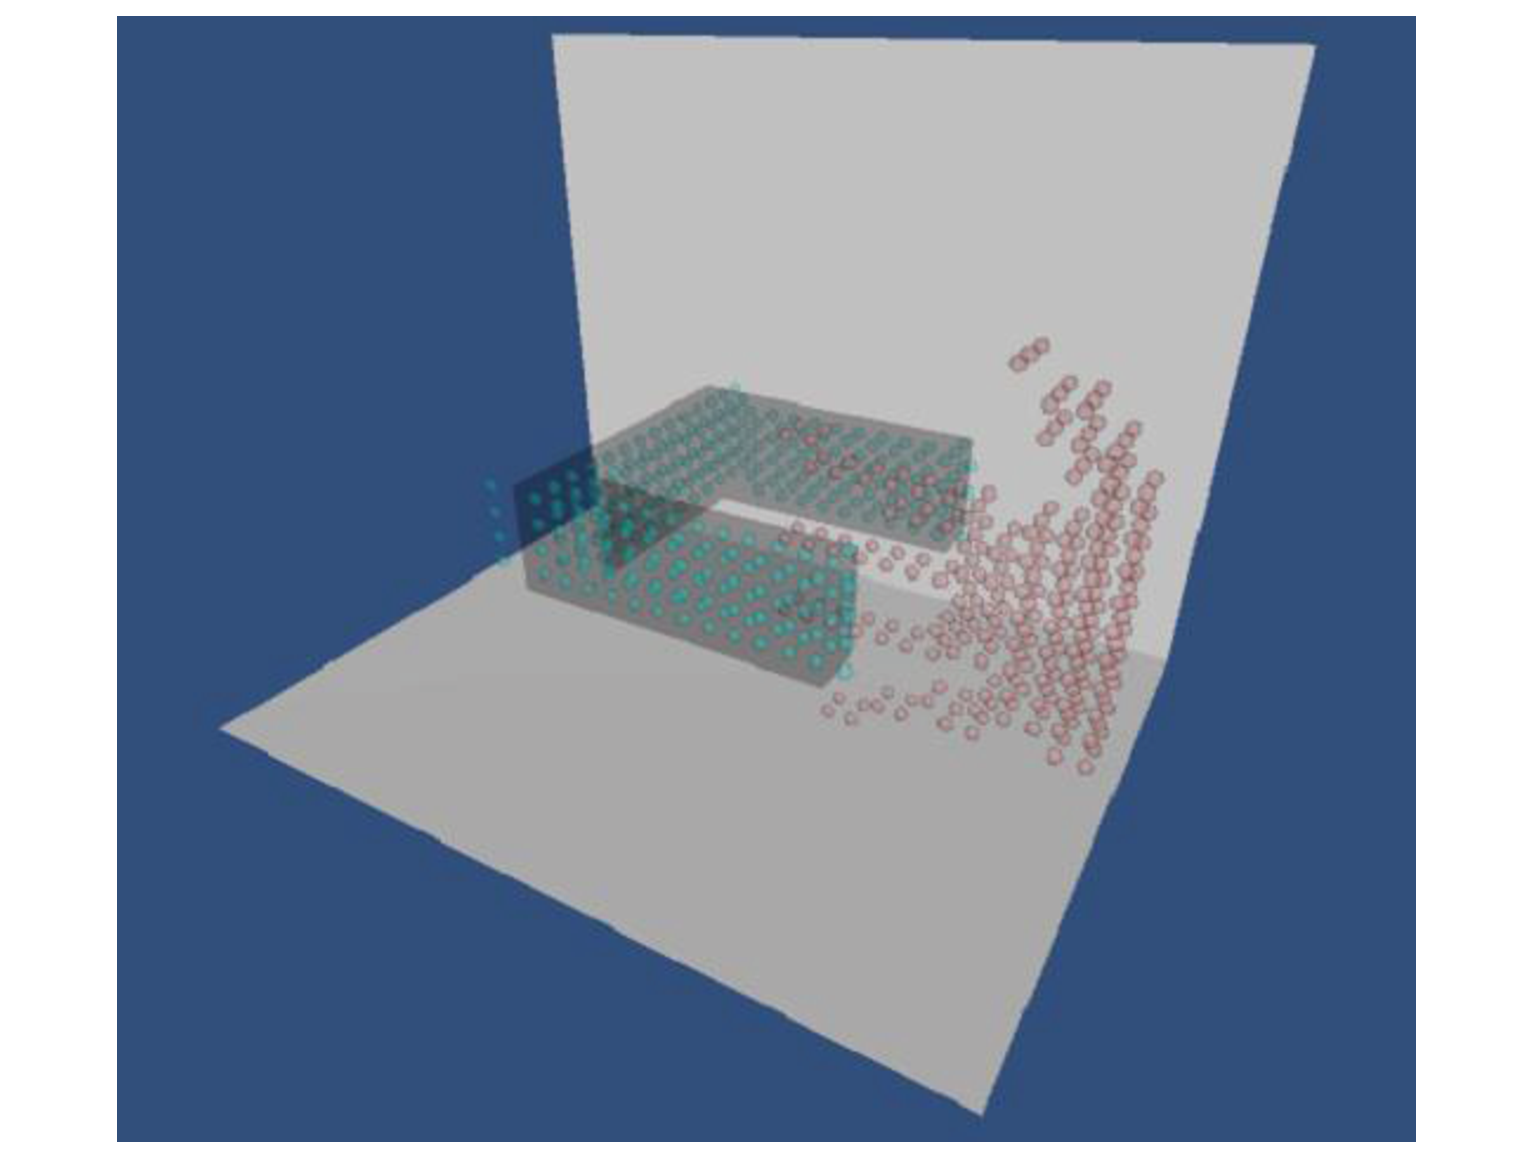
\includegraphics[width=70mm]{3D_obje_insert_2.eps}
   図5-6. 手をオブジェクトの窪みに挿入
  \end{center}
  \label{fig:two}
 \end{minipage}
 
 図5-5、図5-6の赤い点で描写されているものが、手と認識された情報を可視化したものである。窪んだ部分に手を挿入しても、3Dオブジェクトが移動しないことが確認できた。この状態で、手前に動かした結果を図5-7、図5-8に示す。
 
  \vspace{5mm}
\begin{minipage}{0.5\hsize}
  \begin{center}
   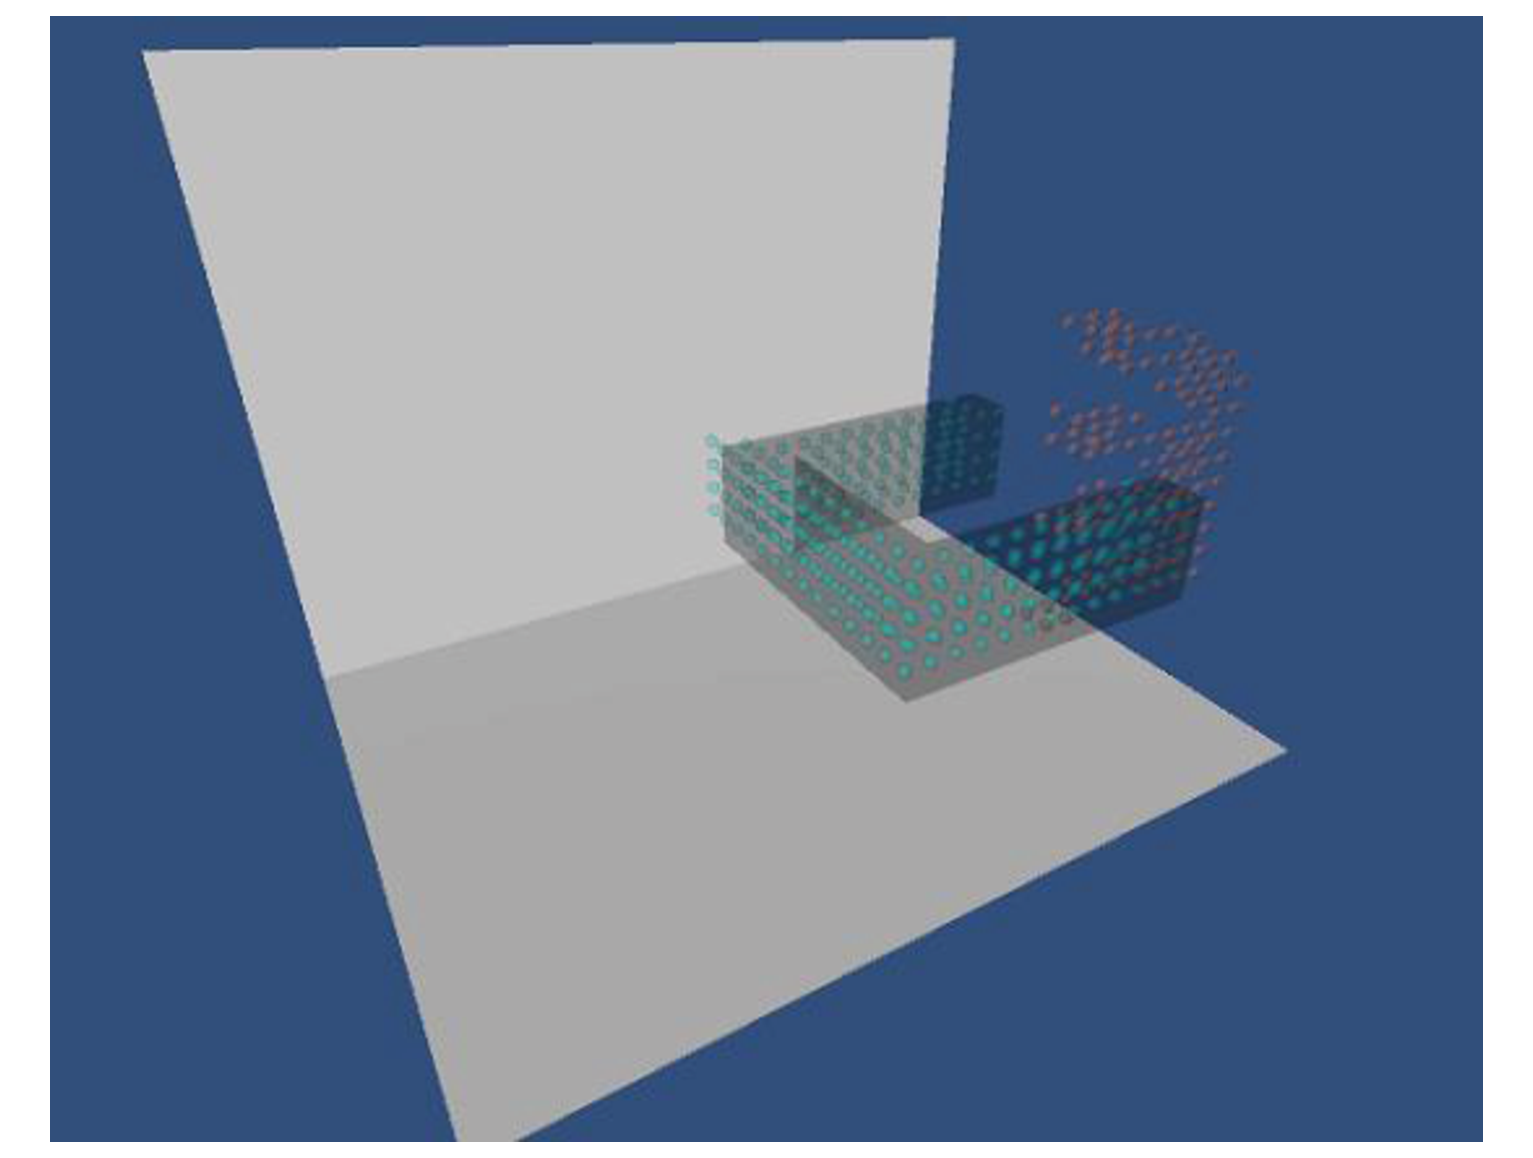
\includegraphics[width=70mm]{temae_1.eps}
   図5-5. 手を手前に移動
  \end{center}
  \label{fig:one}
 \end{minipage}
 \begin{minipage}{0.5\hsize}
  \begin{center}
   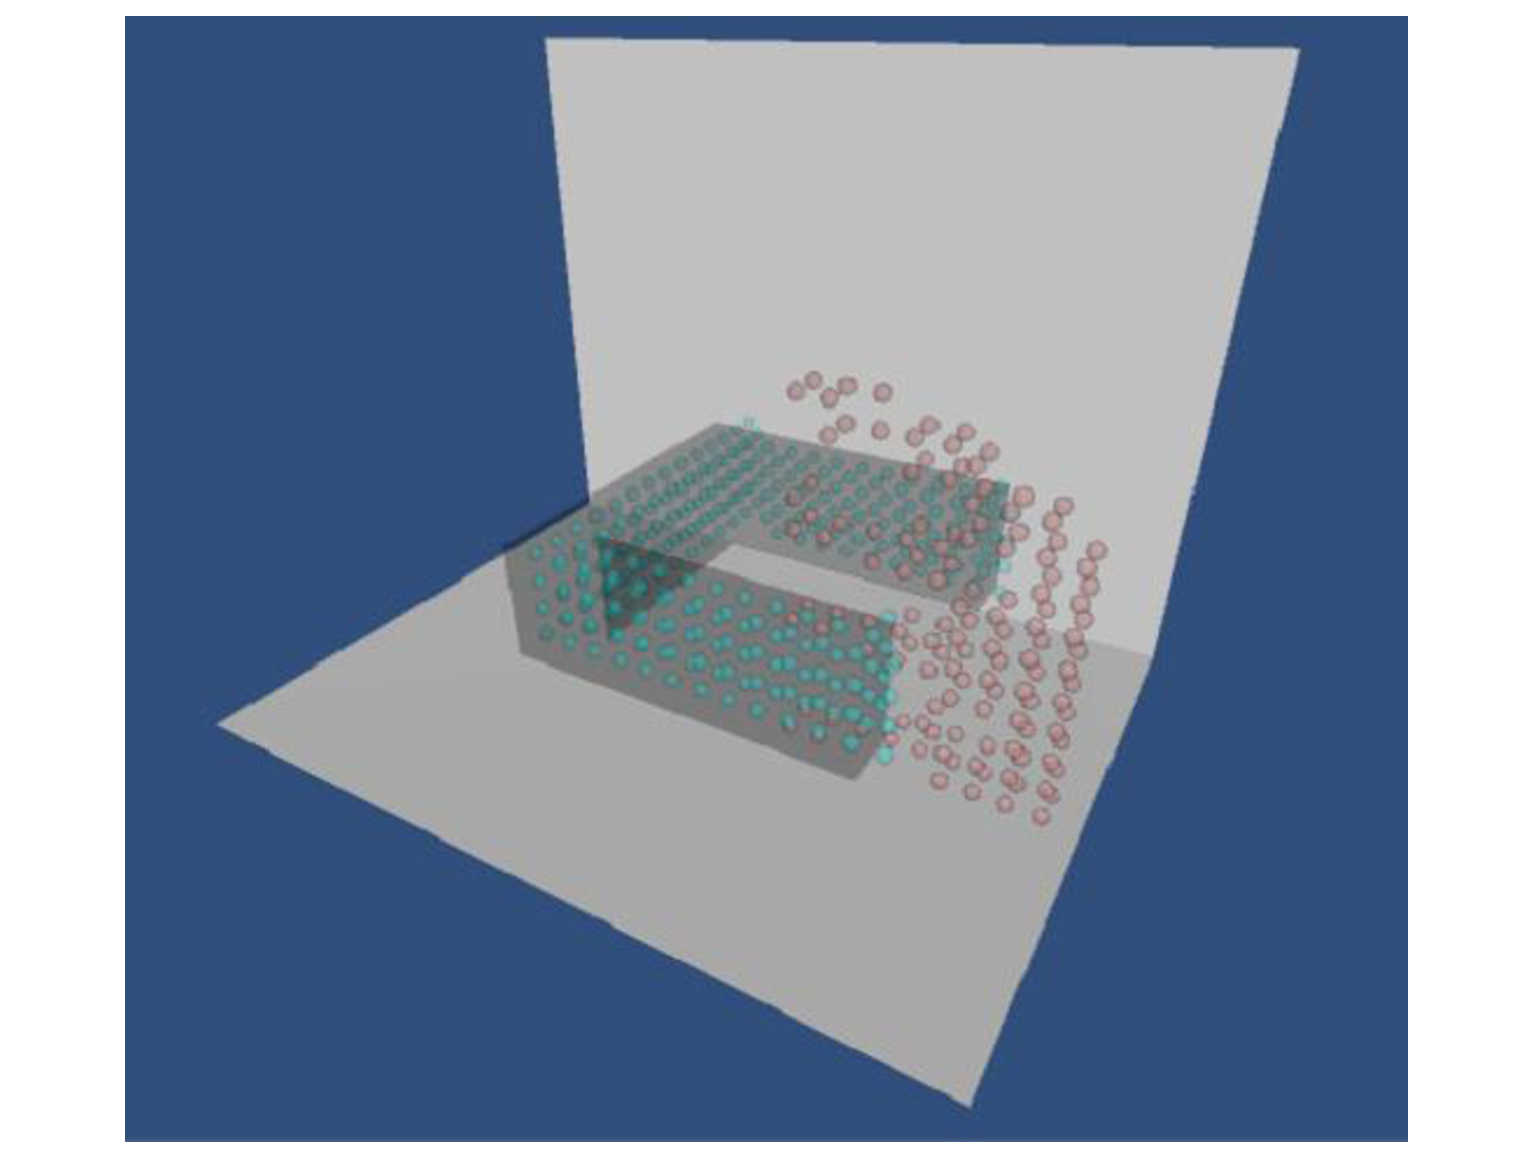
\includegraphics[width=70mm]{temae_2.eps}
   図5-6. 手を手前に移動
     \end{center}
  \label{fig:two}
 \end{minipage}
 
 手がオブジェクトに触れるのと連動して、3Dオブジェクトも手前に移動することが確認できた。これらの結果から、内部外部判定を用いた接触判定は正常に動作していることが確認できる。
 
 
 